\section{System Architecture}
\label{sec:architecture}

IOR is designed as a closed feedback loop. Inference produces an objective estimate;
the divergence between that estimate and the declared purpose steers probing; probe
results provide fresh traces that refine the next round of inference. We describe the
loop as the intended architecture and implement each of its stages, but the present
evaluation exercises the stages individually rather than iterating the full loop;
Section~\ref{sec:limitations} states what closing it would require and the
confirmation-amplifier risk it must control for.

\begin{figure}[h]
\centering
\resizebox{\linewidth}{!}{%
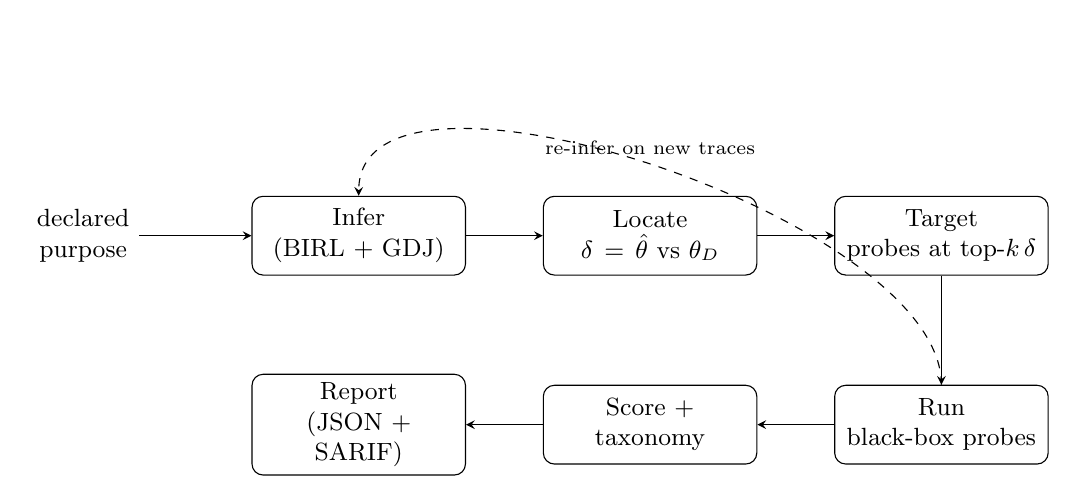
\begin{tikzpicture}[
  font=\small, >=stealth,
  box/.style={draw, rounded corners, align=center, text width=2.5cm,
              minimum height=1cm, inner sep=3pt},
  io/.style={align=center},
]
% top row
\node[io]  (dp)     at (-3.5,0) {declared\\purpose};
\node[box] (infer)  at (0,0)    {Infer\\(BIRL + GDJ)};
\node[box] (locate) at (3.7,0)  {Locate\\$\delta = \hat{\theta}$ vs $\theta_D$};
\node[box] (target) at (7.4,0)  {Target\\probes at top-$k\,\delta$};
% bottom row (right to left)
\node[box] (run)    at (7.4,-2.4) {Run\\black-box probes};
\node[box] (score)  at (3.7,-2.4) {Score +\\taxonomy};
\node[box] (report) at (0,-2.4)   {Report\\(JSON + SARIF)};

\draw[->] (dp) -- (infer);
\draw[->] (infer) -- (locate);
\draw[->] (locate) -- (target);
\draw[->] (target) -- (run);
\draw[->] (run) -- (score);
\draw[->] (score) -- (report);
\draw[->, dashed] (run.north) to[out=90, in=90, looseness=0.7]
  node[pos=0.5, above, font=\scriptsize] {re-infer on new traces} (infer.north);
\end{tikzpicture}%
}
\caption{The IOR closed feedback loop. The solid path runs from the declared purpose
through inference, divergence location, probe targeting, execution, scoring, and
reporting. The dashed arc is the proposed feedback (re-inferring on probe-generated
traces); the present evaluation exercises the solid path only.}
\label{fig:loop}
\end{figure}

The system comprises five modules, summarised in Table~\ref{tab:modules}. The
ingest module validates raw traces into typed trajectory objects. The inference
module recovers a posterior over reward weights. The divergence module ranks the
gap between the inferred and declared objectives. The targeting and execution
modules generate and run probes against the live agent. The scoring and reporting
modules classify findings against regulatory taxonomies and emit machine-readable
reports.

\begin{table}[h]
\centering
\small
\begin{tabular}{@{}llll@{}}
\toprule
Module & Input & Output & Status \\
\midrule
Ingest & Raw log or API trace & Validated trajectory & Complete \\
Infer & Trajectory $+$ declared purpose & $P(\theta \mid \tau)$ via BIRL & Complete \\
Diverge & BIRL result $+$ $\theta_D$ & Ranked $\delta$ & Complete \\
Target $+$ Execute & Ranked $\delta$ & Probe results & Implemented \\
Score $+$ Report & Probe results & JSON $+$ SARIF report & Implemented \\
\bottomrule
\end{tabular}
\caption{The five IOR modules and their Phase~0/1 status.}
\label{tab:modules}
\end{table}

Three design decisions recur throughout the paper. The Goal Decomposition Judge
runs its decomposer once per audit and its critic once per step, with the
decomposition fixed for the duration of an audit so that the same declared purpose
produces the same feature basis (enforced by pinning or caching the goal
specification, since newer models deprecate the temperature parameter that earlier
guaranteed this). The judge model must differ from the agent
under audit to prevent systematic bias alignment. Fast mode uses neutral
counterfactuals rather than scoring every alternative action, trading a quantified
approximation error (Section~\ref{sec:evaluation}) for a large reduction in model
calls.
